\documentclass[a4paper,11pt,fleqn,twoside,openright,final]{memoir}
%%%%%%%%%%%%%%%%%%%%%%%%%%
%% COMMAND DEACTIVATION %%
%%%%%%%%%%%%%%%%%%%%%%%%%%

\let\added\undefined
\let\deleted\undefined


%%%%%%%%%%%%%%
%% PACKAGES %%
%%%%%%%%%%%%%%


%%% Initial things %%%
% Fix various issues with LaTeX2e
\usepackage{fixltx2e}
% Font package
\usepackage{fourier}
% Index
\usepackage{makeidx}
\makeindex


%%% Translations and character encodings %%%
% Enable use of several characters, including æ, ø and å
\usepackage[utf8]{inputenc}
% Danish language
\usepackage[danish]{babel}
% Use PostScript fonts instead of bitmap ones. Also does other stuff.
\usepackage[T1]{fontenc}
% Various LaTeX symbols
\usepackage{latexsym}
% Wider selection of colours
\usepackage[table]{xcolor}
% Improved element justification
\usepackage{ragged2e}
% Font improvements
\usepackage{fix-cm}
% Enables inclusion of PDF files
\usepackage{pdfpages}
% Enables various forms of lines, like double-underlining (\uuline{})
\usepackage[normalem,normalbf]{ulem}
% Sets the tolerance for distance between words, determining when to hyphenate.
\pretolerance=2500


%%% Figures and tables (Floats) %%%
% Ensures that floats won't appear -before- the place where they're added
\usepackage{flafter}
% Enable multi-rows and -columns
\usepackage{multirow}
\usepackage{multicol}
% Double, horizontal lines
\usepackage{hhline}
% Enables coloured tables
\usepackage{colortbl}
% Gives improved control over placement of floats
% \begin{figure}[!h] % Won't be floating
\usepackage{here}
% Wrap text around figures
\usepackage{wrapfig}
% Wrap text around tables
\usepackage{floatflt}
% Enables the \FloatBarrier command
\usepackage{placeins}
% Rotation of figures
\usepackage{rotating}
% Framed boxes
\usepackage{framed}
% Booktabs - Fancy tables
\usepackage{booktabs}
% Enables inclusion of PDF documents of version 1.6+
\pdfoptionpdfminorversion=6


%%% Mathematic formulas %%%
% AMS math
\usepackage{amsmath}
\usepackage{amssymb}
% Extra fonts (for math, I think)
\usepackage{stmaryrd}
% Access text symbols
\usepackage{textcomp}
% Extend AMS
\usepackage{mathtools}
\usepackage{cancel}
% Use theorems in your document
% The ntheorem package is also used for the example environment
% When using thmmarks, amsmath must be an option as well. Otherwise \eqref doesn't work anymore.
\usepackage[framed,amsmath,thmmarks]{ntheorem}
% Pretty fractions, just because
\usepackage{nicefrac}


%%% Graphics %%%
% Various image-commands
\usepackage{eso-pic}
% Use JPEG and PNG images
\usepackage{array,graphicx}
\DeclareGraphicsExtensions{.pdf,.png,.jpg}
\graphicspath{{./images/}}
%Wrapping Images
\usepackage{wrapfig}


%%% Text stuff %%%
% Filler text
\usepackage{lipsum}
% Page counting
\usepackage{totpages}
% Acronyms
\usepackage{acronym}
%avoid widows
\widowpenalty10000


%%% Source Code Stuff %%%
% Adds \lstinline!code there!, where !! are delimeters not used in the code
% Adds the environment: lstlisting
% Adds command \lstinputlisting[options]{filename.ext}
% More info in manual.
%\usepackage{listings}
%\lstloadlanguages{[Sharp]C,XML,SQL}
%\lstset{numbers=left,
%        numberstyle=\tiny,
%        stepnumber=2,
%        numbersep=5pt,
%        frame=tb,
%        inputencoding=utf8,
%        tabsize=2,
%        extendedchars=true,
%        language=[Sharp]C}

\usepackage{color}
\definecolor{bluekeywords}{rgb}{0.13,0.13,1}
\definecolor{greencomments}{rgb}{0,0.5,0}
\definecolor{redstrings}{rgb}{0.9,0,0}

\usepackage{courier}

\usepackage{listings}

\lstdefinelanguage{JavaScript}{
  keywords={typeof, new, true, false, catch, function, return, null, catch, switch, var, if, in, while, do, else, case, break},
  keywordstyle=\color{blue}\bfseries,
  ndkeywords={class, export, boolean, throw, implements, import, this},
  ndkeywordstyle=\color{darkgray}\bfseries,
  identifierstyle=\color{black},
  sensitive=false,
  comment=[l]{//},
  morecomment=[s]{/*}{*/},
  commentstyle=\color{purple}\ttfamily,
  stringstyle=\color{red}\ttfamily,
  morestring=[b]',
  morestring=[b]"
}


\lstset{language=[Sharp]C,
  captionpos=b,            
  columns=fixed,     
  numbers=left,
  numberstyle=\tiny,
  showspaces=false,
  showtabs=false,
  breaklines=true,
  inputencoding=utf8,
  showstringspaces=false,
  breakatwhitespace=true,
  escapeinside={(*@}{@*)},
  commentstyle=\color{greencomments},
  keywordstyle=\color{bluekeywords},
  stringstyle=\color{redstrings},
  basicstyle=\ttfamily\small,
  literate={ø}{{\o}}1
  		   {æ}{{\ae}}1
  		   {å}{{\aa}}1
  		   {Ø}{{\O}}1
  		   {Æ}{{\AE}}1
  		   {Å}{{\AA}}1
}

\lstdefinestyle{make}{tabsize=4}

%%% References, bibtex and URLs %%%
% Post URLs. Allows breaking at hyphens to help avoid long links.
\usepackage[hyphens]{url}
% Better cross references
\usepackage[danish]{varioref}
% Enable natbib citation styles
\usepackage[numbers]{natbib}
% Define a new 'leo' style for URL package, that will use a smaller font
\makeatletter
\def\url@leostyle{%
  \@ifundefined{selectfont}{\def\UrlFont{\sf}}{\def\UrlFont{\small\ttfamily}}
}
\makeatother
% And of course, use this new style
\urlstyle{leo}




%%% Floats %%%
% Not entirely sure why I need this yet
\let\newfloat\relax
\usepackage{float}
% Enables usage of \subcaption, \subtop and \subbottom
\newsubfloat{figure}


%%% Todo Stuff %%%
% Insert needed corrections with \fixme{..}, which will cause an error during compile, if any are present once 'draft'
% is replaced with 'final'
\usepackage[footnote,draft,danish,silent,nomargin]{fixme}
\fxsetup{layout={footnote,marginclue,index},innerlayout={inline,index}}


%%% Changes Markup %%%
% Markup changes of varying types.
% Adds the commands:
%  - \added[id=(author id), remark={remark text}]{new text}
%  - \deleted[id=(author id), remark={remark text}]{old text}
%  - \replaced[id=(author id), remark={remark text}]{new text}{old text}
\usepackage[xcolor,authormarkup=footnote]{changes}
% Adds the commands:
%  - \cbstart
%  - \cbend
%  - \cbdelete
%  - Environment: changebar
\usepackage[outerbars,xcolor]{changebar}
\cbcolor{red}



%%%%%%%%%%%%%%%%%%%%%%%
%% DOCUMENT SETTINGS %%
%%%%%%%%%%%%%%%%%%%%%%%


%%% Margins %%%
% \setlrmarginsandblock{binding}{edge}{ratio}
\setlrmarginsandblock{3.5cm}{2.5cm}{*}
% \setulmarginsandblock{top}{bottom}{ratio}
\setulmarginsandblock{2.5cm}{3.0cm}{*}
% Performs various calculations and makes several non-Memoir things work with the Memoir class
\checkandfixthelayout 
% Correct todonotes placement
\reversemarginpar


%%% Paragraph formatting %%%
% Size of paragraph indentation
\setlength{\parindent}{0mm}
% Distance between paragraphs (double enter)
\setlength{\parskip}{3mm}
% Line distance
\linespread{1,1}


%%% Bibliography %%%
% Defines parameters for the bibliography, such as the parenthesis and separators
%%%% OLD STYLE!
%\bibpunct{[}{]}{,}{a}{}{;}
% Bibliography style
%%%% OLD STYLE!
%\bibliographystyle{bibtex/harvard}
\bibliographystyle{plainnat}


%%% Table of contents %%%
% Depth of numbered headlines
\setsecnumdepth{subsubsection}
% Changing the document class' limit for number-depth
\maxsecnumdepth{subsection}
% Define the depth included in the table of contents
\settocdepth{section}
% Use letters instead of Roman numerals in TOC
\renewcommand{\thepart}{\Alph{part}}


%%% Text stuff %%%
% Removes distance between items in itemize
%\let\olditemize=\itemize
%\def\itemize{\olditemize\setlength{\itemsep}{-1ex}}
%% Removes distance between items in enumerate
%\let\oldenumerate=\enumerate
%\def\enumerate{\oldenumerate\setlength{\itemsep}{-1ex}}
\usepackage{enumitem}


%%% Changes (Language strings) %%%
\addto\captionsdanish{
  \def\listofchangesname{Ændringer i dokumentet}
  \def\summaryofchangesname{Ændringer}
  \def\changesaddname{Tilføjet}
  \def\changesdeletename{Slettet}
  \def\changesreplacename{Erstattet}
  \def\changesauthorname{Skribent}
  \def\changesanonymousname{anonym}
  \def\changesnoloc{Listen af ændringer tilgængelig efter næste \LaTeX\ kørsel.}
  \def\changesnosoc{Opsummering af ændringer tilgængelig efter næste \LaTeX\ kørsel.}
}


%%% Visual references %%%
% Enables clickable hyperlinks
\usepackage[colorlinks,hidelinks,backref=page]{hyperref}
% General setup of hyperlinks package
\hypersetup{
    breaklinks = true,
    colorlinks = false,
    linkcolor = black,
    anchorcolor = black,
    citecolor = black
}


%%% Colour definitions %%%
% Defines: gray
\definecolor{gray}{gray}{0.80}
% Defines: numbercolor
\definecolor{numbercolor}{gray}{0.7}
% Defines: shadecolor
\definecolor{shadecolor}{RGB}{33,26,82}
% Defines: aaublue
\definecolor{aaublue}{RGB}{33,26,82}


%%% Figure and table texts setup %%%
% Font definition for the 'Figure' or 'Table' displays.
\captionnamefont{\small\bfseries\itshape}
% Font definition for the numbering
\captiontitlefont{\small}
% Delimiter between number and figure text
\captiondelim{. }
% Left justify multi-line figure texts below one another
\hangcaption
% Width of figure text
\captionwidth{\linewidth}
% Distance below figure text
\setlength{\belowcaptionskip}{10pt}
% Fix space between figure number and name
\setlength{\cftfigurenumwidth}{14mm}


%%% Page header and footer %%%
% Define width of header and footer
\setlength{\headwidth}{\textwidth}
% Create pagestyle for pages with and without a new chapter
\makepagestyle{reportPlain}
\makepagestyle{reportChapter}
% Pagestyle for chapter pages (Only a footer, of course)
\makefootrule{reportChapter}{\headwidth}{\normalrulethickness}{\footruleskip}
\makeevenfoot{reportChapter}{\thepage}{}{}
\makeoddfoot{reportChapter}{}{}{\thepage}
% Pagestyle for regular pages
\makerunningwidth{reportPlain}{\headwidth}
\makeheadposition{reportPlain}{flushright}{flushleft}{flushright}{flushleft}
\makeevenhead{reportPlain}{\leftmark}{}{}
\makeoddhead{reportPlain}{}{}{\rightmark}
\makeevenfoot{reportPlain}{\thepage}{}{}
\makeoddfoot{reportPlain}{}{}{\thepage}
\makeheadrule{reportPlain}{\headwidth}{\normalrulethickness}
\makefootrule{reportPlain}{\headwidth}{\normalrulethickness}{\footruleskip}
% Use pagestyles
\pagestyle{reportPlain}
\aliaspagestyle{chapter}{reportChapter}
\aliaspagestyle{part}{reportChapter}
\aliaspagestyle{title}{empty}
% Do not stretch pages
\raggedbottom


%%% Naming %%%
% Define various names for captions and such
\addto\captionsdanish{
  \renewcommand\appendixname{Bilag}
  \renewcommand\contentsname{Indholdsfortegnelse} 
  \renewcommand\appendixpagename{Bilag}
  \renewcommand\cftchaptername{\chaptername~}
  \renewcommand\cftappendixname{\appendixname~}
  \renewcommand\appendixtocname{Bilag}
}


%%% Appendix setup %%%
% Appendix setup. Might need some settings here
\usepackage{appendix}


%%% Chapter look and feel %%%
% Define style: jenor
\newif\ifchapternonum
\makechapterstyle{jenor}{
  \renewcommand\printchaptername{}
  \renewcommand\printchapternum{}
  \renewcommand\printchapternonum{\chapternonumtrue}
  \renewcommand\chaptitlefont{\fontfamily{pbk}\fontseries{db}\fontshape{n}\fontsize{25}{35}\selectfont\raggedleft}
  \renewcommand\chapnumfont{\fontfamily{pbk}\fontseries{m}\fontshape{n}\fontsize{1in}{0in}\selectfont\color{numbercolor}}
  \renewcommand\printchaptertitle[1]{%
    \noindent
    \ifchapternonum
    \begin{tabularx}{\textwidth}{X}
    {\let\\\newline\chaptitlefont ##1\par}
    \end{tabularx}
    \par\vskip-2.5mm\hrule
    \else
    \begin{tabularx}{\textwidth}{Xl}
    {\parbox[b]{\linewidth}{\chaptitlefont ##1}} & \raisebox{-15pt}{\chapnumfont \thechapter}
    \end{tabularx}
    \par\vskip2mm\hrule
    \fi
  }
}
% Use style: jenor
\chapterstyle{jenor}


%%%%%%%%%%%%%%%%%%%%%%%%%%%%%%%%%%%%%%%%%%%%%%%%
% An example environment (http://kom.aau.dk/~jkn/latex/latex.php)
%%%%%%%%%%%%%%%%%%%%%%%%%%%%%%%%%%%%%%%%%%%%%%%%
\theoremheaderfont{\normalfont\bfseries}
\theorembodyfont{\normalfont}
\theoremstyle{break}
\def\theoremframecommand{{\color{aaublue!50}\vrule width 5pt \hspace{5pt}}}
\newshadedtheorem{exa}{Eksempel}[chapter]
\newenvironment{example}[1]{%
		\begin{exa}[#1]
}{%
		\end{exa}
}


%%% Misc stuff %%%
% Use regular numbers for pages
\pagenumbering{arabic}
% Word and letter counts
\newcommand{\wordcount}{\input{preamble/sums/wordcount.sum}}
\newcommand{\charcount}{\input{preamble/sums/charcount.sum}}
\newcommand{\lettercount}{\charcount}
\newif\ifcounts
% Italicized quote-environment
\newenvironment{italicquote}{\begin{quote}\itshape}{\end{quote}}
% Acronyms in list or not (true if in list)
\newif\ifAcroList
\AcroListfalse


%%% Left-aligning bibliography %%%
%\renewcommand*{\bibfont}{\raggedright}


%%%% these patches ensure that the backrefs point to the actual occurrences of the citations in the text, not just the page or section in which they appeared
%%%% http://tex.stackexchange.com/questions/54541/precise-back-reference-target-with-hyperref-and-backref
%%%% BEGIN BACKREF DIRECT PATCH, apply these AFTER loading hyperref package with appropriate backref option
% The following options are provided for the patch, currently with a poor interface!
% * If there are multiple cites on the same (page|section) (depending on backref mode),
%   should we show only the first one or should we show them all?
\newif\ifbackrefshowonlyfirst
\backrefshowonlyfirstfalse
%\backrefshowonlyfirsttrue
%%%% end of options
%
% hyperref is essential for this patch to make any sense, so it is not unreasonable to request it be loaded before applying the patch
\makeatletter
% 1. insert a phantomsection before every cite, so hyperref has something to target
%    * in case natbib is loaded. hyperref provides an appropriate hook so this should be safe, and we don't even need to check if natbib is loaded!
\let\BR@direct@old@hyper@natlinkstart\hyper@natlinkstart
\renewcommand*{\hyper@natlinkstart}{\phantomsection\BR@direct@old@hyper@natlinkstart}% note that the anchor will appear after any brackets at the start of the citation, but that's not really a big issue?
%    * if natbib isn't used, backref lets \@citex to \BR@citex during \AtBeginDocument
%      so just patch \BR@citex
\let\BR@direct@oldBR@citex\BR@citex
\renewcommand*{\BR@citex}{\phantomsection\BR@direct@oldBR@citex}%

% 2. if using page numbers, show the page number but still hyperlink to the phantomsection instead of just the page!
\long\def\hyper@page@BR@direct@ref#1#2#3{\textit{\hyperlink{#3}{Side #1}}}

% check which package option the user loaded (pages (hyperpageref) or sections (hyperref)?)
\ifx\backrefxxx\hyper@page@backref
    % they wanted pages! make sure they get our re-definition
    \let\backrefxxx\hyper@page@BR@direct@ref
    \ifbackrefshowonlyfirst
        %\let\backrefxxxdupe\hyper@page@backref% test only the page number
        \newcommand*{\backrefxxxdupe}[3]{#1}% test only the page number
    \fi
\else
    \ifbackrefshowonlyfirst
        \newcommand*{\backrefxxxdupe}[3]{#2}% test only the section name
    \fi
\fi

% 3. now make sure that even if there is no numbered section, the hyperref's still work instead of going to the start of the document!
\RequirePackage{etoolbox}
\patchcmd{\Hy@backout}{Doc-Start}{\@currentHref}{}{\errmessage{I can't seem to patch backref}}
\makeatother
%%%% END BACKREF PATCHES


% Enable figures like checkmarks
\usepackage{pifont}
\newcommand{\cmark}{\ding{51}}%
\newcommand{\xmark}{\ding{55}}%

%%%%%%%%%%%%%%%%%%%%%%%%%%%%%%%%%%%%%%%%%%%%%%%%
%Flowchart
\usepackage{tikz}
\usetikzlibrary{shapes.geometric, arrows, positioning}
%%%%%%%%%%%%%%%%%%%%%%%%%%%%%%%%%%%%%%%%%%%%%%%%

%\usepackage{bera}% optional: just to have a nice mono-spaced font

\newcommand*\rot{\rotatebox{90}}

\colorlet{punct}{red!60!black}
\definecolor{background}{HTML}{EEEEEE}
\definecolor{delim}{RGB}{20,105,176}
\colorlet{numb}{magenta!60!black}

\lstdefinelanguage{json}{
    basicstyle=\normalfont\ttfamily,
    numbers=left,
    numberstyle=\scriptsize,
    stepnumber=1,
    numbersep=8pt,
    showstringspaces=false,
    breaklines=true,
    frame=lines,
    backgroundcolor=\color{background},
    literate=
     *{:}{{{\color{punct}{:}}}}{1}
      {,}{{{\color{punct}{,}}}}{1}
      {\{}{{{\color{delim}{\{}}}}{1}
      {\}}{{{\color{delim}{\}}}}}{1}
      {[}{{{\color{delim}{[}}}}{1}
      {]}{{{\color{delim}{]}}}}{1},
}
% Preamble additions
%%%% Acronyms %%%

% Add acronyms here, using \acrodef{acronym}[short name]{full name}
%   or \acro{acronym}[short name]{full name}
% Afterwards, these can be referred to as \ac{acronym}

\begin{acronym}
\end{acronym}

%%% Changes (Authors) %%%
\definechangesauthor[name={Mathias Corlin Mikkelsen}, color=orange]{CK}
\definechangesauthor[name={Marc Thorgersen}, color=blue]{MT}
\definechangesauthor[name={Morten Pedersen}, color=brown]{NS}
\definechangesauthor[name={Mathias Sass Michno}, color=olive]{TN}
\definechangesauthor[name={Troels Krøgh}, color=teal]{TK}
\definechangesauthor[name={Søren Frandsen}, color=violet]{SF}

% Define valid hyphenations in cases where TeX falls short
\hyphenation{hvad hvem hvor}

% Comment out the following to remove word and letter counts
\countstrue
% Reference definition
\usepackage[danish]{cleveref}
\crefname{exa}{eksempel}{eksempler}
\newcommand{\myref}[1]{\vref{#1}}
\newcommand{\Myref}[1]{\Vref{#1}}
\begin{document}
\sloppy
% Front matter starts here
\frontmatter
% Insert front page
%\thispagestyle{empty}

%\AddToShipoutPicture*{\put(0,0){
\includegraphics{images/frontpage.pdf}}}

%\hphantom{ }

%  A simple AAU report template.
%  2013-03-06 v. 1.0.0
%  Copyright 2010-2013 by Jesper Kjær Nielsen <jkn@es.aau.dk>
%
%  This is free software: you can redistribute it and/or modify
%  it under the terms of the GNU General Public License as published by
%  the Free Software Foundation, either version 3 of the License, or
%  (at your option) any later version.
%
%  This is distributed in the hope that it will be useful,
%  but WITHOUT ANY WARRANTY; without even the implied warranty of
%  MERCHANTABILITY or FITNESS FOR A PARTICULAR PURPOSE.  See the
%  GNU General Public License for more details.
%
%  You can find the GNU General Public License at <http://www.gnu.org/licenses/>.
%
\thispagestyle{empty}
\pdfbookmark[0]{Front page}{label:frontpage}%
  \addtolength{\hoffset}{0.5\evensidemargin-0.5\oddsidemargin} %set equal margins on the frontpage - remove this line if you want default margins
  \noindent%
  \begin{tabular}{@{}p{\textwidth}@{}}
    \toprule[2pt]
    \midrule
    \vspace{0.2cm}
    \begin{center}
    \Huge{\textbf{
      P3: ProjectFood% insert your title here
    }}
    \end{center}
    \begin{center}
      \Large{
        - Udvikling af applikationer \\fra brugere til data, algoritmer og test\\ og tilbage igen -% insert your subtitle here
      }
    \end{center}
    \vspace{0.2cm}\\
    \midrule
    \toprule[2pt]
  \end{tabular}
  \vspace{2cm}
  \begin{center}
    {\large
      Projektrapport%Insert document type (e.g., Project Report)
    }\\
    \vspace{0.2cm}
    {\Large
      DS304E14%Insert your group name or real names here
    }
		\vspace{2 cm}
		\begin{flushleft}
			\parindent=2 cm
			\Large
      \begin{minipage}{0.45\textwidth}
      \centering
      \rule{\textwidth}{0.5pt}\\
			\textit{Mathias Corlin Mikkelsen}
      \end{minipage}
		\end{flushleft}
		\begin{flushright}
			\hangindent=2 cm
			\Large
      \begin{minipage}{0.45\textwidth}
      \centering
      \rule{\textwidth}{0.5pt}\\
			\textit{Marc Tom Thorgersen}
		  \end{minipage}
    \end{flushright}
		\begin{flushleft}
			\parindent=2 cm
			\Large
      \begin{minipage}{0.45\textwidth}
      \centering
      \rule{\textwidth}{0.5pt}\\
			\textit{Morten Pedersen}
		  \end{minipage}
    \end{flushleft}
		\begin{flushright}
			\hangindent=2 cm
			\Large
      \begin{minipage}{0.45\textwidth}
      \centering
      \rule{\textwidth}{0.5pt}\\
			\textit{Mathias Sass Michno}
		  \end{minipage}
    \end{flushright}
		\begin{flushleft}
			\hangindent=2 cm
			\Large
      \begin{minipage}{0.45\textwidth}
      \centering
      \rule{\textwidth}{0.5pt}\\
			\textit{Søren Hvidberg Frandsen}
		  \end{minipage}
    \end{flushleft}
		\begin{flushright}
			\hangindent=2 cm
			\Large
      \begin{minipage}{0.45\textwidth}
      \centering
      \rule{\textwidth}{0.5pt}\\
			\textit{Troels Beck Krøgh}
		  \end{minipage}
    \end{flushright}

  \end{center}
  \vfill
  \begin{center}
  Aalborg Universitet\\
  Institut for datalogi\\
  Selma Lagerlöfs Vej 300\\
  9220 Aalborg Ø
  \end{center}
%\clearpage

% Ensure that next page opens on the right
\cleardoublepage
% Insert title page
\thispagestyle{empty}
\enlargethispage*{\ifcounts 4\else 2\fi\baselineskip}
{\samepage
\begin{tabular}{cc}
  \parbox{0.5\textwidth}{ %
    \hspace*{1cm} %
    
\includegraphics[width=4cm,height=4cm,keepaspectratio]{images/aau_logo_da.pdf}} &
  \parbox{0.5\textwidth}{\begin{tabular}{l}
      {\small \textbf{3. Semester --- Software}}\\
      {\small Selma Lagerlöfs Vej 300} \\
      {\small 9210 Aalborg SØ} \\
      {\small http://www.cs.aau.dk/}
    \end{tabular}}
\end{tabular}

\begin{tabular}{cc}
  \parbox{8cm}{
  \begin{description}
    \item { \textbf{Titel:}}\\ 
      ProjectFood
    \item { \textbf{Tema:}}\\ 
      Programering og modelløsning. 
  \end{description}
  
  \parbox{8cm}{
  \begin{description}
    \item { \textbf{Projektperiode:}}\\
      P3 (Efterårssemestret 2014) \newline 02-09-2014 - 19-12-2014
    \hspace{4cm}
    \item { \textbf{Projektgruppe:}}\\
        DS304E14
    \hspace{4cm}
    \item {\textbf{Gruppemedlemmer:}}\\
      Marc Tom Thorgersen\\
      Søren Hvidberg Frandsen\\
      Troels Beck Krøgh\\
      Mathias Corlin Mikkelsen\\
      Morten Pedersen\\
      Mathias Sass Michno\\
    \hspace{2cm}
    \item { \textbf{Vejleder:}}\\
      Thomas Bøgholm\\
    \end{description}
  }

  \begin{description}
    \item { \textbf{Oplagstal:} x}
    \item { \textbf{Rapport sideantal:} x} 
    \item { \textbf{Appendiks sideantal:} x}
    \item { \textbf{Total sideantal:} \ref{TotPages}}
    \item { \textbf{Projekt klaret den:}\\ 19-12-2014} 
    \ifcounts
      \item { \textbf{Ord/Tegn (Cirka):} ...}
    \fi
  \end{description}
  \vfill } &
  \parbox{7cm}{
   \vspace{.15cm}
    \hfill 
    \begin{tabular}{l}
      { Abstract:}\bigskip \\
      \fbox{
      \parbox{6.5cm}{\bigskip
        {\vfill{\small % Abstract indeholder beskrivelse af opgaven, formål/problemstilling, anvendte metoder, resultater
% og konklusioner.

The following project studies how to fuk
        \bigskip}}
      }}
    \end{tabular}}
\end{tabular}
}%samepage end
\\
\vfill
\noindent{\footnotesize{\textit{Rapportens indhold er frit tilgængeligt, men offentliggørelse (med kildeangivelse) må kun ske efter aftale med forfatterne.}}}
% Ensure that next page opens on the right
\cleardoublepage
%StateOfTheArt.tex
% Insert foreword
%\chapter{Forord}

\lipsum*[1]


%\cleardoublepage
% Insert table of contents
\thispagestyle{empty}
\tableofcontents*
\label{table_of_contents}
%%%%%%%%%%%%%%
%% CHAPTERS %%
%%%%%%%%%%%%%%
% Main matter starts here
\mainmatter
\part{Analyse}
\chapter{Indledning}\label{chapter:indledning}

I dagligdagen kan det være svært at koordinere indkøb, opskrifter og tilbud således, at dette foregår på en optimal måde. Nogle kigger i tilbudsaviser og planlægger deres indkøb i en eller flere butikker, andre vælger kun at handle i en butik. Hvis ikke man planlægger disse indkøbsture, kan det lede til madspild pga. overindkøb/impulskøb eller for mange unødige ture i supermarkederne, hvilket kan tage tid i ens hverdag. Derudover kan det være problematisk at koordinere, hvem der handler hvad ind med eventuelle samboende.  

Det kan også være svært at leve sundt og varieret som fødevareministeriet foreslår; det kan være svært at finde på noget at lave til aftensmad; eller også har man ikke nogen gode opskrifter, man synes om. 
Hvis man planlægger sine indkøb efter opskrifter, skal man holde styr på, hvilke varer man har i sit hjem for at undgå at købe for meget ind. Det kan samtidig være svært at overskue, hvilken butik der er den bedste at handle ind i på et givent tidspunkt, eftersom at tilbud hele tiden ændrer sig og faste priser er forskellige. Det er heller ikke sikkert, at den valgte opskrift man køber ind efter, indeholder varer, som er på tilbud, når man gerne vil have dem - på denne måde ender man måske med at leve dyrere end nødvendigt. 

Dette projekt vil undersøge, om man kan gøre det nemmere at handle efter tilbuddene i dagligvarebutikkerne, alt imens man reducerer problemerne vedr. det at beslutte sig for, hvad man skal lave til aftensmad. 
Derfor vil der i de følgende afsnit blive udforsket hvad der er på markedet til hjælp med denne problemstilling. Desuden vil der også undersøges personers vaner, samt holdninger til elektronisk hjælp til problemstillingen i form af korte interviews.

\chapter{Læsevejledning}
Her vil komme tekst om læsevejledning.

Teksten vil beskrive kildehenvisninger, samt kodeeksempler.

Ord som 'vi' referer til forfatterne af rapporten.

 Eventuel beskrivelse af struktur på: CD, bilag og andet.

\chapter{State of the art}
I dette afsnit vil løsningerne der allerrede findes på markedet bliver udforsket.
Der vil blive kigget på web services og applikationer der har til samme formål at løse nogle af de samme problemer vi undersøger nærmere.
Løsningerne der er præsenteret, hjælper med de problemer beskrevet i \myref{chapter:indledning}

\section{eTilbudsavisen}
eTilbudsavis er en online service der kan findes på \url{http://www.eTilbudsavis.dk}. eTilbudsavis er en online avis med en høj funktionalitet og en nem brugergrænseflade.
Der kan på siden oprettes et login, således der kan findes tilbage til ændringer på et senere tidspunkt eller andre enheder.
eTilbudsavis har tre mærkbare funktioner som brugeren har adgang til, hvilket er tilbudsaviser, ønske- og indkøbslister og tilbud.

Tilbudsaviser kan tilgås på siden, hvor der er mulighed for at sætte en præference på, hvor store en radius man vil lede efter sagte tilbudsavis. 
Der kan der vælges imellem alle aviser, som er tilgængelige online og inden for den valgte radius. 
Aviserne bliver opdateret løbende, så når der er en ny tilgængelig bliver den gamle fjernet. 
Inde i aviserne kan man trykke på en vare og den bliver tilføjet til en liste.

Der er mulighed for at tilføje vare til to lister, en indkøbsliste og en ønskeliste. 
Når en vare er valgt bliver den tilføjet til den valgte liste.
Listen indeholder navn, butik, pris og den valgt mængde, for varen. 
Der kan foruden at vælge varer fra tilbudsaviserne, nemt skrives generiske varer på listen. Varen på listen kan da krydses af for at kunne holde styr på hvad der er blevet købt.

Hvis det ikke ønskes at skulle bladres tilbudsaviser igennem, er der den mulighed at få vist en hel side kun med tilbud. 
Alle aktuelle tilbud fra aviserne, er da vist som elementer med navn, beskrivelse, pris, butik, og afstand. Disse tilbud kan på samme måde nemt tilføjes til listerne.

eTilbudsavis er en god online løsning som har mange gode features, derfor har vi også brugt dem som kilde til vores tilbud, dette API er beskrevet i Kapitel \ref{api}.

\section{Tilbudsugen}

Tilbudsugen minder på mange måder om eTilbudsavis. 
Den har samtlige dagligvareaviser, samt flere inden for bl.a. Byggemarkeder, og Autoudstyr.
De giver et nemt overblik over diverse aviser, og man kan hurtigt og nemt læse dem på nettet. 
Der er desuden mulighed for at lave præferencer som ved eTilbudsavis, her kan man bl.a. vælge økologi eller nøglehulsmærket.
Når man tilføjer en vare til indkøbslisten, søger den automatisk efter tilbud på den valgte vare. 
Man bliver bedt om at vælge et specifikt tilbud, og netop dette tilbud bliver tilføjet til indkøbslisten, med pris, butik, udløbsdato, mængde, og et billede af varen.
Man kan som i eTilbudsavis også trykke på en vare direkte i avisen, for at tilføje den til sin liste.
Hvis man vil dele sin indkøbsliste er det også en mulighed vha. en ``delekode'' som man kan give til en anden bruger, og de kan på denne måde også se listen.
Funktionerne findes på hjemmesiden, men det er ikke altid de virker, for eksempel hvis man tilføjer noget uden at angive et antal, og du så prøver at dele listen med en, vil de ikke være at finde på listen.
Desuden kan man ikke ændre på antallet af varen du allerede har sat på din indkøbsliste. 
For at opnå dette skal man slette varen, og tilføje den igen med det nye antal.
De har desuden også en smartphone app, men denne crasher ofte når man benytter sig af deres indkøbsliste, men fungerer tilgengæld fint hvis man blot vil se på ugens tilbud i aviserne.

\section{Smartphone Apps udgivet af butikker}
På \myref{tbl-smartphone} ses der nogle butikskæder som har udviklet android apps, og hvilke funktionaliteter disse har.  
For at skabe et overblik er der udvalgt features og disse er blevet opsat i et skema for overskuelighed. 
\begin{table}[H]
	\centering
		\colorlet{shadecolor}{gray!40}
    	\rowcolors{1}{white}{shadecolor}
	    \begin{tabular}{l|lllllllllll}
	    %Table: http://bit.ly/1tD6EI6
	   	%Funktionalitet & Tilbudsavis & Indkøbsliste & Opskrifter & Varescan & Find butik & Budget & Madplan & Rabatkupon/fordelsordning & Deling af indkøbslister & Rating på Play & Senest opdateret \\ \hline
	     & \rot{Tilbudsavis} & \rot{Indkøbsliste} & \rot{Opskrifter} & \rot{Varescan} & \rot{Find butik } & \rot{Budget} & \rot{Madplan} & \rot{Rabatkupon} & \rot{Deling} & \rot{Play rating} & \rot{Senest} \rot{opdateret} \\ \hline
	   	Føtex                       & \cmark   & \cmark    & \cmark  & \cmark   & \cmark  & ~      & ~       & ~          & ~                       & 3.4 (354)      & 2014-07-24       \\
	    SPAR                        & \cmark   & \cmark    & \cmark  & ~        & \cmark  & \cmark & ~       & ~          & ~                       & 2.8 (64)       & 2014-05-15       \\
	    Fakta                       & \cmark   & \cmark    & \cmark  & ~        & \cmark  & ~      & \cmark        & \cmark     & \cmark               & 3.1 (454)      & 2014-08-02       \\
	    FaktaQ                      & \cmark   & ~         & \cmark  & ~        & \cmark  & ~      & ~       & ~          & ~                       & 4.4 (7)        & 2014-03-11       \\
	    REMA 1000                   & \cmark   & \cmark    & \cmark  & ~        & \cmark  & ~      & ~       & ~          & ~                       & 3.5 (674)      & 2014-04-16       \\
	    SuperBrugsen                & \cmark   & \cmark    & \cmark  & ~        & \cmark  & ~      & ~       & ~          & ~                       & 3.8 (987)      & 2014-06-30       \\
	    Kvickly                     & \cmark   & \cmark    & \cmark  & ~        & \cmark  & ~      & ~       & ~          & ~                       & 3.7 (632)      & 2014-07-20       \\
	    \end{tabular}
	    \caption{Nogle butikskæder med smartphone apps samt deres funktionaliteter.}\label{tbl-smartphone}
	\end{table}
Vi har valgt at undersøge en af disse apps nærmere, og valget faldte på Faktas app,
da denne bliver opdateret og har flest funktioner. 
\subsection{Faktas Android App}\fxnote{Screenshot?}
Faktas android app kalder de for ``Mit fakta'', den er som helhed overskuelig.
Efter åbning af appen har man mulighed for seks menupunkter og at ændre sine indstillinger.
Første menupunkt omhandler ``Coop-kortet'' og giver bruger mulighed for at indtaste sine medlemsinfomationer, da disse giver særlige tilbud.
Andet menupunkt er deres tilbudsavis, hvilket blot er en digital kopi af den fysiske tilbudsavis. 
Dog kan man fra den også tilføje varer til sin indkøbsliste, eller se varerne i et gitterformat.
Tredje menupunkt er ``indkøbsliste'', her kan man have flere personlige og/eller delte indkøbslister.
Her kommer deres Facebook integration også i spil, og tillader nem deling af indkøbsliste med brugerens Facebook venner.
Fjerde menupunkt er en madplan, hvori man kan planlægge sin egen madplan, eller se Faktas anbefalinger til en under 20 kr pr. person pr. aften.
Femte menupunkt er deres opskrifter.
Her findes der et stort antal af opskrifter, disse kan tilføjes direkte til sin madplan eller indkøbslister (både personlige og delte).
Sjette menupunkt hedder ``Åbningstider'', her kan brugeren finde Faktas butikker og deres åbningstider. \fxnote{Fungerer det godt? Hvad fungerer skidt? - Søren}


\section{Tøm køleskabet}
Der findes talrige tjenester, der tilbyder “at tømme dit køleskab”. 
Mere specifikt, tilbyder de en service, hvor du som bruger, angiver hvilke varer dit køleskab pt. indeholder, samt hvilke andre ingredienser du har til rådighed. 
Derefter får du så præsenteret en række forskellige opskrifter, der kan laves ud fra dine tilgængelige ingredienser. 
De fleste af tjenesterne (herunder dem vi her har undersøgt) viser også opskrifter, som indeholder yderligere ingredienser. 
Dette betyder naturligvis, at man som bruger ikke bliver fritaget fra at handle ind, hvis man mangler nogle ingredienser til lige netop den opskrift, man vælger at udføre. 
Tjenesten \textit{MyFridgeFood} \footnote{kan findes på \underline{www.myfridgefood.com}} tilbyder, at oprette en indkøbsliste ud fra netop disse manglende ingredienser, hvilket kan lade sig gøre blandt andet fordi, alle opskrifter er interne på \textit{MyFridgeFood}. 
I modsætning til dette er der \textit{Supercook} \footnote{kan findes på \underline{www.supercook.com}}, som linker til eksterne opskrifter, og ikke tilbyder at generere en indkøbsliste. 
Umiddelbart anbefales opskrifter ikke ud fra den enkelte brugers smag og madvaner, men udelukkende på baggrund af, hvad man “har i køleskabet”. 
Grundet dette virker tjenesterne mere som simple filtreringer af databaseopslag, end egentlige anbefalinger, der tager højde for brugerens smag og præferencer indenfor den gastronomiske verden.

\section{Alternativer til Indkøbsturen}
Der findes altså allerede mange applikationer, i form af apps til smartphones og webapps, som kan hjælpe med indkøbsturen og planlægning af måltider. Hvis disse indeholder opskrifter som tager højde for tilbudene i en given uge, er det inden for en enkelt butikskædes tilbud. Der er altså ingen applikationer der tager højde for tilbud fra alle butikskæderne. I dette afsnit undersøges der alternativer til indkøbsturen.

Ud over mobilapplikationer, flytter nogle dagligvarebutikker på internettet, sådan man kan handle ind hjemmefra, som man kender det fra almindelig nethandel.
Andre løsninger er baseret på abonnementsordninger, som fjerner meget af planlægningen fra ordningens bruger.
Herunder gennemgås eksempler på nogle firmaer der tilbyder de to ovennævnte løsninger.

De seneste år har online dagligvare-butikker skudt frem, og selvom de er i kraftig vækst udgør de kun en lille del af det samlede dagligvareforbrug i Danmark\citep{SOTA_MP1}.

\subsection{Online butikker}
Eksempler på online dagligvarebutikker er SuperBest og Irma\citep{SOTA_MP_SB, SOTA_MP_IRMA}.
Nogle af butikkerne har dog kun en online butik, og ingen fysisk modpart, dette er butikker som Nemlig.com og Osuma\citep{SOTA_MP_NEMLIG, SOTA_MP_OSUMA}.
Disse butikker kan gøre det lettere at handle ind.
Sådanne butikker giver både mulighed for at handle ind hjemmefra eller fra studiet eller arbejde i en pause.
Ved at handle hjemmefra kan man også let overskue hvad man mangler imens man handler ind, og man kan derfor undgå at glemme at skrive noget på indkøbssedlen.
Ligeledes undgår man at stå i supermarkedet og være i tvivl om man mangler en bestemt vare.
Nogle af firmaerne tilbyder også opskrifter.
Nemlig.com tilbyder opskrifter og hjemmesiden kan præsentere alle deres varer som indgår i listen over ingredienser.
Dette gør at man direkte fra en given opskrift kan sammenligne tilsvarende varer, og tilføje en af dem til sin indkøbskurv.
Andre butikker giver også mulighed for at oprette madplaner, hvilket kan gøre planlægningen af indkøb og madlavning i hjemmet, lettere.
Disse online butikker kommer dog også med forskellige ulemper i forhold til fysiske supermarkeder.
Det koster penge at få leveret sine varer fra disse butikker, typisk omkring 50 kr. og i nogle af butikkerne skal man købe for et minimumsbeløb.
Ved handel gennem online butikkerne, kan du ikke få varerne med det samme, det variere butikkerne i mellem, hvor stor ventetiden er.
Disse to ulemper gør ligeledes at man ikke kan benytte disse løsninger hvis man står og mangler en vare eller to. \fxfatal{Men hvis man var hardcore bruger af disse services, ville man jo være i stand til at planlægge forud og totalt ungå denne, ellers ret normale, situaltion? - Troels}


\subsection{Abonnementsordninger}
Ordningerne sender typisk kasser med daglivarer ud til deres kunder.
Disse kassers indhold tilbyder ofte en varieret blanding af kød, grønt og frugt.
I denne kategori findes udbydere som Aarstiderne og igen SuperBest\citep{SOTA_MP_AAR, SOTA_MP_SB}.
Ideen med sådanne kasser er at nogle ansatte, typisk kokke eller lignende, ved eksempelvis Aarstiderne har sammensat kasser med ingredienser til 3-5 aftensmåltider.
På deres hjemmeside eller mobilappikation kan man så finde guide og opskifter til hvordan maden tilberedes.
Derudover har Aarstiderne også suppleret med ydeligere tre kategorier, for at tilbyde mere fleksible løsninger til kunderne.
Den første kategori holder sig inde for kasse-dogmet, og er generelle kasser, hvor man eksempelvis kan købe en kødkasse, fiskekasse eller en frugtkasse, i disse kategorier findes der så forskellige kasser inden for hver kategori.
Anden kategori er supplering hvorigennem kunderne kan købe forskellige varer i løssalg, hvis ikke kasserne opfylder deres behov.
Sidste kategori er morgenmad, her tilbyer de en blanding mellem kasser og løssalg.
Denne model kan løse mange problemer i forhold til madlavningen for kunderne.
Løsningen vil kunne mindske den planlægning en person behøves at foretage sig, fordi kasserne indeholder alle ingredienser til flere måltider, samt opskrifter at følge.
Dette betyder at kunden  hverken behøves at planlægge aftensmaden eller indkøbet dertil.
Ligeledes ville den kraftigt mindske behovet for at handle ind andre steder.
Denne løsning kommer dog heller ikke uden ulemper.
Dogmet med at forudbestemme flere måltider og have de eksakte ingredienser begrænser den kreativitet som en person normalt ville kunne udleve i køkkenet.
Ydermere begrænses ideen meget af den moderne families struktur, hvor det ofte ikke er hele familien der spiser sammen, mange dage om ugen. \fxfatal{En kilde på dette? - Troels}
Det er også svært at tage højde for præferencer som kræsenhed eller allergier i disse forudbestemte kasser.
Denne løsning vil heller ikke kunne fritage en bruger fra at skulle handle ind andre steder end her, da de ikke tilbyder alt.

Som vi har set i ovenstående gennemgang, findes der alternativer til den klassiske indkøbstur, der er dog ingen af disse der formår at løse alle problemerne.
Ved alle løsningerne opstår også nye ulemper og problemstillinger i forhold til almindeligt indkøb.
Alt taget i betragtning vil det komme meget an på nuværende vaner og familiestrukturen, om disse muligheder vil være en god løsning for en given familie.


\chapter{Indledende interview}
Onsdag d. 17 september gennemførte vi en række semi-strukturerede interviews i Aalborg midtby blandt folk omkring Føtex. Vi adspurgte syv personer i forskellige målgrupper, herunder unge der bor alene, unge der bor sammen med nogen, og  folk over 30 med begge førnævnte sociale statusser. Aldersspændet var fra 20 - 51, og kønnene var ligeligt fordelt. Formålet med disse interviews var at danne et basalt overblik over vores problemområde, samt undersøge, hvordan folk håndterede vores initierende problem på nuværende tidspunkt. Vores interviews bestod af en håndfuld forberedte spørgsmål, samt løsere samtale, for at følge op på disse spørgsmål. Ud af interviewene fandt vi følgende hovedpunkter:
\begin{itemize}
	\item Generelt er folk uorganiserede når det kommer til indkøb, og især unge mennesker bruger sjældent indkøbslister.
	\item Inspiration til aftensmåltider findes ofte i indkøbssituationen eller ud fra princippet “hvad man lige har lyst til”.
	\item Det er ikke mange, der gennemgår tilbudsaviser, og endnu færre går bevidst efter tilbud. Dog kan det påvirke beslutninger om aftensmåltid, hvis en given varer er på tilbud i butikken, hvor der handles ind.
	\item Især den yngre målgruppe (18-28) er interesseret i en løsning med tilbud, indkøbslister og opskrifter til inspiration kædet sammen. Mens den ældre målgruppe (28+) virker mere interesseret i at kunne dele indkøbslister med familie, for bedre at kunne organisere indkøb.
	\item Opskrifter er som sagt noget, der mest interesserer det yngre segment. Dog påpeger nogle, at stor tendens til at være kræsen kræver at man kan sætte præferencer. 
\end{itemize}

Dog skal det nævnes, at en mere dybdegående undersøgelse samt analyse vil være nødvendig, for at kunne beslutte design elementer og videre systemkrav.     Fremadrettet vil der arbejdes videre med følgende områder:

\begin{itemize}
	\item Indkøbslister
	\item Tilbud
	\item Opskrifter.
\end{itemize}

\chapter{Systemdefinition}
Ud fra problemformuleringen og det hidtige arbejde udarbejdes en BATOFF-analyse, som beskrevet i OOA\&D\citep{OOA&D2001} og efterfølgende formuleres en skreven systemdefinition baseret på disse kriterier.

Denne analyse har til formål at definerer retningen for det videre arbejde i projektet.
Dette gøres ved at beskrive nogle overordnet tanker om programmet ud fra de seks BATOFF-kritirier.

Nedenfor ses BATOFF udarbejdlsen og efterfølgende systemdifinitionen.

\section{BATOFF}

\begin{description}
\item [Betingelser]\hfill
\begin{itemize}
\item Adgang til tilbud (API)
\item Interesse for indkøb, opskrifter og tilbud
\end{itemize}

\item [Anvendelsesområde]\hfill
\begin{itemize}
\item eTilbudsavis
\item Brugere
\item Servere
\item Klienter
\item Overvågning af tilbud og madvaner
\item Midler til lagring af data
\item Styring af anbefalinger
\end{itemize}

\item [Teknologi]\hfill
\begin{itemize}
\item Smartphone (Mobil web-device)
\item Til udvikling: Computer m/udviklerværktøjer
\item Browser m/internetadgang
\end{itemize}

\item [Objekter]\hfill
\begin{itemize}
\item Opskrifter
\item Indkøbsvarer (tilbud)
\item Brugere
\item Vurdering 
\item Præferencer
\item Indkøbsliste
\item Tilbudsaviser 
\end{itemize}

\item [Funktioner]\hfill
\begin{itemize}
\item Overvågning af varer 
\item Håndtering af indkøbslister
\item Bedømmelse af opskrifter
\end{itemize}

\item [Filosofi]\hfill
\begin{itemize}
\item Indkøbsassistent og inspirationsgenerering
\end{itemize}
\end{description}

 



Disse kriterier, hjælper med at danne overblik over diverse emner der bør berøres i en systemdefinition, og på det grundlag er følgende systemdefinition udarbejdet:

\section{Systemdefinition}

Systemet hjælper på problemer, der kan opstå i forbindelse med indkøb og madlavning i hjemmet. 
Systemet organiserer indkøbslister, opskrifter og aktuelle tilbudsvarer, samt anbefaler varer og/eller opskrifter, baseret på tidligere valg, bedømmelser af opskrifter og præferencer ang. madvarer. 
Aktuelle tilbud hentes fra internettet, og kan tilføjes, sammen med generiske varer, til indkøbslister, samt overvåge hvornår, en bestemt type vare kommer på tilbud.
Systemet tilgås via en webbrowser, således der kan bruges både computer, tablet og smartphone. 
Systemet vil blive udviklet som en serverside-applikation med adgang til databaser til håndtering af system- og brugerdata. 
Udviklingen af systemet kræver computere med de relevante udviklingsværktøjer.\\

Denne systemdefinition vil nu være udgangspunkt for vores videre arbejde i rapporten.
\chapter{Problem- og Anvendelesområdeanalyse}

I forhold til vores projekt om opskriftsanbefalinger og indkøbsassistent er der flere objekter som skal analyseres i forhold til henholdsvis problemområdet samt andvejdelsesområdet.

\section{Problemområde analyse}
Problemområdet defineres som:

\textit{``Den del af omgivelserne, der administreres, overvåges eller styres ved hjælp af et system.''}

Personer som er relevante for vores produkt er personer som laver mad og handler ind i hjemmet, disse vil have noget besvær med minimum en af følgende ting, finde relevante tilbud, finde på retter at lave til aftensmad, handle ind til bestemte retter, bruge og følge indkøbssedler.
Disse personer betegner vi som kunder.

Opskrifter er objekter i problemområdet da dette er noget som den enkelte kunder benytter sig af under tilberedningen af mad.
Opskrifter har forskellige ingredienser der skal tages højde for når kunderne har deres præferencer som veganisme eller allergier.
Ligeledes opererer brugerne indkøbslister til at holde styr på hvad der skal købes ind.
Disse indkøbslister kan ofte være inspireret af tilbud de forskellige supermarkeder har en given uge.
Varene er et objekt der skal kunne overvåges da brugeren har mulighed for at overvåge en specifik vare og dens pris, dette hænger sammen med de tilbud der føres på de givne varer samt hvilke varer der bliver brugt i de forskellige opskrifter.
Kunderne er objekter i den forstand at de foretager sig valg af varer på indkøbslister og valg af opskrifter at bruge, disse valg og handlinger skal overvåges for at tilpasse vores anbefalinger af opskrifter og tilbud.
Der er mulighed for at kunder deler login og hver kunde kan have forskellige præferencer, navn, diæt osv.
Vurderingerne som brugerne har foretaget under brug af systemet, vil blive anvendt til at anbefale nye opskrifter, varer og tilbud.

\begin{itemize}
	\item Opskrifter
	\item Tilbud
	\item Indkøbsliste
	\item Varer
	\item Kunder
	\item Vurderinger 
\end{itemize}
                                                                                                                                                                                                   
\section{Anvendelseområde analyse}
Anvendelsesområdet defineres som:

\textit{``En organisation, der administrerer, overvåger eller styrer et problemområde.''}

eTilbudsavis er en organisation der overvåger tilbudsaviser der er tilgængelige online, og giver da mulighed for at foretage søgninger og fremfinde præcise tilbud ud fra en større samling af aviser.
Denne information skal vi bruge til at kunne informere brugerne om relevante tilbud.
Derfor har vi taget kontakt til eTilbudsavisen, og håber på at få lov til at bruge deres API.
Brugerne er personer der overvåger varer, opretter indkøbslister og ser på tilbud samt bedømmer opskrifter.
Brugerne administrerer også hvilke krav og præferencer de har til deres indkøbsliste og derfor også deres opskrifter.
De reagere på og overvåger derfor også anbefalinger som andre brugere har vurderet.
En server skal overvåge og administrere anbefalinger, kunder og databaser.
Serveren skal sørge  for at kunderne har adgang til deres data fra forskellige enheder.
Serveren vil give anbefalinger ved at sammenligne de vurderinger en opskrift har modtaget fra flere brugere.

Klienter er de enheder kunder benytter til at tilgå servicen, dette kan være smartphones eller computere.

\begin{itemize}
	\item eTilbudsavis
	\item Brugere
	\item Server
	\item Klienter (desktop, smartphone)
\end{itemize}

\chapter{Data-Flow diagram}
\begin{figure}
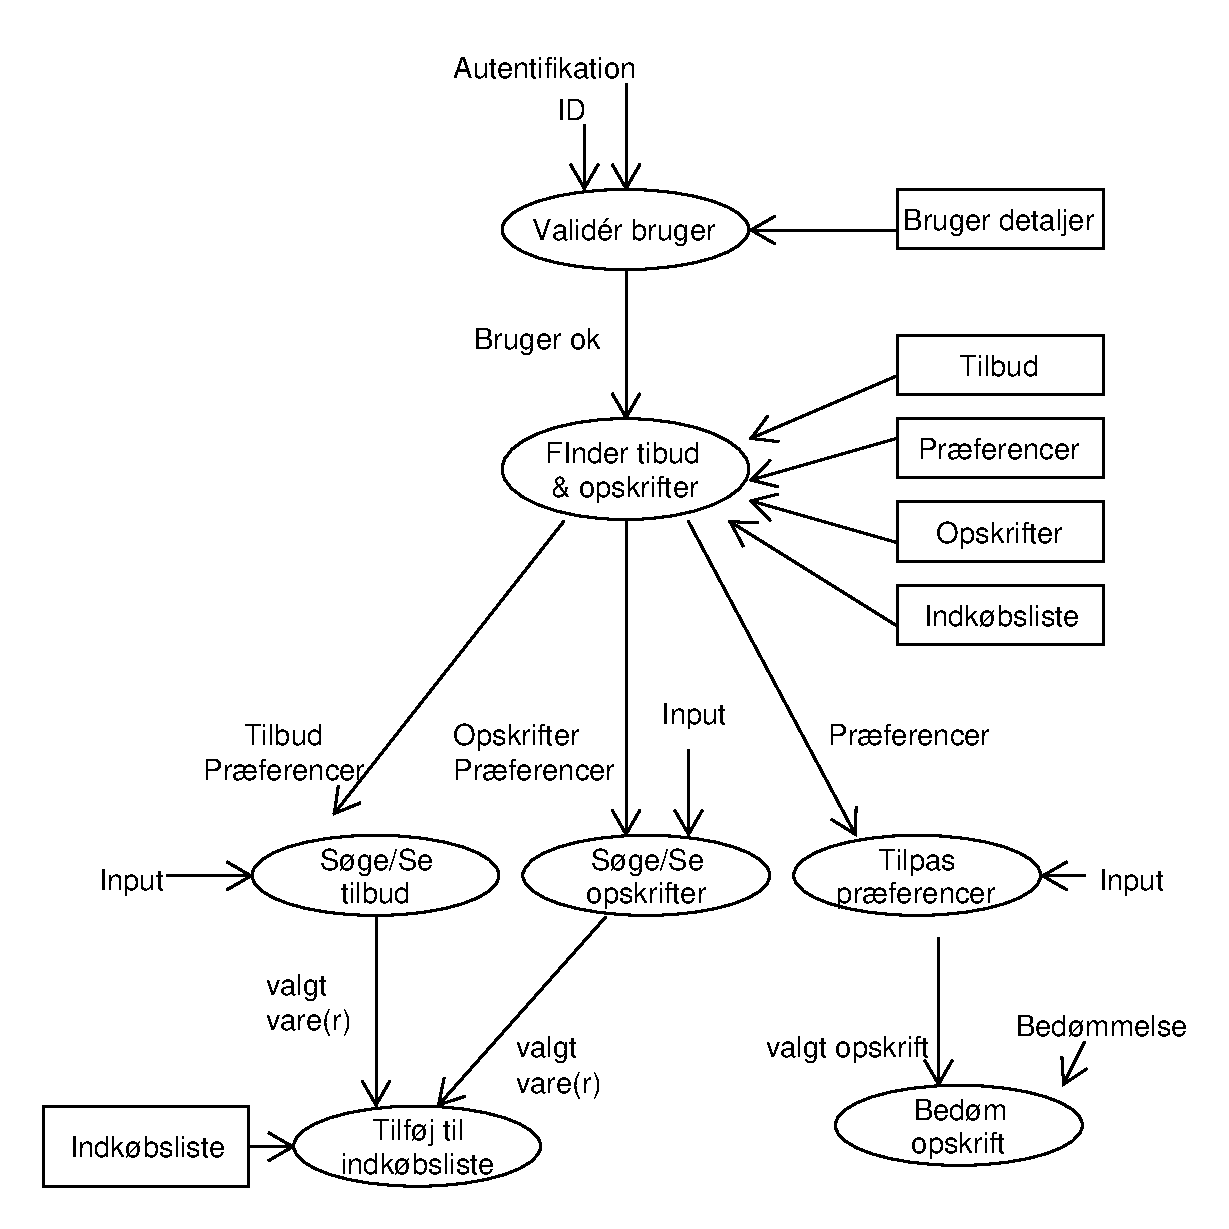
\includepdf[scale=0.75]{images/Diagrams/Dataflowdiagram_0.pdf}
\end{figure}
\chapter{PACT}

\section{Personer}
Majoriteten af personerne, som anvender systemet, har interesse i at lave mad i husstanden, og hjælpe med indkøb til madlavningen.
Brugerne af systemet er hovedsageligt voksne mennesker, hvilket betyder, at alle har et grundlag for at læse simpel tekst i systemet.
Der tages hermed ikke hensyn til blinde, og folk med voldsomme læsevanskeligheder.
Personerne, der benytter systemet, forventes ligeledes at kunne forstå dansk.
Mere specifikt er personerne meget forskellige.
Det kan både være enlige, samboende, unge og gamle, og systemet kan også bruges af hele familier.
Personerne kan også være kræsne eller have forskellige krav(herunder bl.a. allergier) og præferencer, i forhold til mad og madvaner.

\section{Aktiviteter og kontekst}
Aktiviteterne er delt op i to dele, da der vil være to delløsninger. 
Den ene vil være delen med opskrifter og tilbudssøgning, imens den anden er indkøbslisten.
Samtidigt er konteksten og delt op i to: her handler det om, at systemet kan bruges i hjemmet, men også at det kan bruges i selve indkøbsøjeblikket, altså i supermarkedet.
Systemet skal kunne tilgås let som indkøbsliste, og således også være let brugbart i et indkøbscenter, mens der handles ind.
Indkøbslisten skal derfor være nem at komme til og synkronisere i realtime.
Man skal kunne sætte ting på indkøbslisten i det øjeblik, man kommer i tanke om, at man mangler dem.
I konteksten af hjemmet, behøver systemet ikke være lige så øjeblikkelig, da man som oftest har mere tid til at tænke over sine valg.
Dog er det altid vigtigt, at systemet er responsivt i alle kontekster og ved alle aktiviteter, for ikke at ødelægge den pågældende aktivitets flow. 

\section{Teknologier}
For at et software system skal være brugbart som indkøbsliste, kræves det, at platformen er portabel.
Der sættes således et krav om, at systemet vil være brugbart på en mobil platform som smartphones.
Yderligere indebærer problemet et fokusområde, som omhandler tilbud, opskrifter og præferencer.
Disse vil oftere være nemmere tilgængeligt via en enhed med en større skærm, såsom en computer eller tablet - men vil med fordel også kunne tilgås ved brug af en smartphone. 	
\chapter{Konceptuelle scenarier}

%\chapter{Kravspecifikation}
Formål: Et formelt dokument som fortæller hvilke funktioner som det endelige produkt skal have. 

\section{Krav til systemet}
\begin{enumerate}
	\item Systemet skal tilgås ved brug af en internetbrowser, altså skal det være en web-app.
	\item Systemet skal benytte aktuelle tilbud fra diverse dagligvarebutikker.
	\item Systemet skal have mulighed for at overvåge tilbud på varer valgt af slutbrugeren.
	\item Systemet skal have mulighed for at indeholde en personlig indkøbsliste
	\begin{enumerate}
		\item Integreret med tilbud.
		\item Indkøbslisten deles mellem enheder
		\item Indkøbslisten deles mellem brugere fra samme husstand. 
	\end{enumerate}
	\item Systemet skal kunne præsentere opskrifter for brugere.
	\begin{enumerate}
		\item Systemet skal kunne modtage feedback på de opskrifter brugerne giver.
		\item Systemet skal kunne anbefale opskrifter på baggrund af:
		\begin{enumerate}
			\item Madvaner (varieret kost)
			\item Bedømmelse på opskrift
		\end{enumerate}
	\end{enumerate}
	\item Systemet skal have en række præferencer pr. bruger.
	\begin{enumerate}
		\item Systemet skal kunne fjerne forslag om eksempelvis kød til vegetarer.
	\end{enumerate}
\end{enumerate}
\section{Krav til brugergrænsefladen (“UI”)}
\begin{enumerate}
	\item Systemets UI skal være på dansk.
	\item Systemet skal kunne anvendes på forskellige enheder\fxfatal{Vi har nogle steder inkluderet tablets i denne liste, er de med eller ej? - Troels}
	\begin{enumerate}
		\item Computere, > 11” og > 768 px i højden og > 1280 px i breden.
		\item Smartphones, < 6”
	\end{enumerate}
	\item Systemets UI skal være responsivt og tilpasse sig den anvendte platform.
	\item Systemets UI skal anvende design principperne “proximity” og “consistency”.
	\item Systemets UI skal anvende en top-menu til den øverste hierarkiske navigation. 
	\begin{enumerate}	
		\item Top-menuen skal være tilgængelig fra alle sider i applikationen. 
	\end{enumerate}
	\item Systemets UI skal anvende direct mapping, dvs. ikoner somrepræsenterer handlinger (metafor).
	\item Systemet skal tilbyde en fortryd-knap, i henhold til princippet “Effectiveness”.
\end{enumerate}


%\makeatletter\@openrightfalse
%\let\cleardoublepage\clearpage
%\part{Problemløsning}
%\makeatletter\@openrightfalse
%\let\cleardoublepage\clearpage
%\part{Refleksion}
%%%%%%%%%%%%%%%%
%% REFERENCES %%
%%%%%%%%%%%%%%%%
%\backmatter
\makeatletter\@openrightfalse
\let\cleardoublepage\clearpage
\part{Referencer}
%%% Bibliography %%%
\bibliography{bibtex/litteratur}
%%% Figures %%%
%\newpage
%\listoffigures
%%% Tables %%%
%\listoftables
%%% Acronyms %%%
\vspace*{18mm}
\@openrighttrue\makeatother
%%%%%%%%%%%%%%
%% APPENDIX %%
%%%%%%%%%%%%%%
%\part{Appendiks}
%\appendix
%\settocdepth{chapter}
%\chapter{Test}

%%%%%%%%%
% INDEX %
%%%%%%%%%
\newpage
\printindex
\end{document}